%%%%%%%%%%%%%%%%%%%%%%%%%%%%%%%%%%%%%%%%%%%%%%%%%%%%%%%%%%%%%%%%%%%%%%%%%%%%%%%%%%
\begin{frame}[fragile]\frametitle{}
\begin{center}
{\Large Introduction to Probability distributions}
\end{center}
\end{frame}


%%%%%%%%%%%%%%%%%%%%%%%%%%%%%%%%%%%%%%%%%%%%%%%%%%%%%%%%%%%
\begin{frame}
\frametitle{Probability distributions}
The probability distribution for a random variable X gives the possible 
values for X, and the probabilities associated with each possible value 
(i.e., the likelihood that the values will occur). 
Types:
\begin{itemize}
\item Discrete probability distributions 
\item Continuous probability distributions 
\end{itemize}
\end{frame}

%%%%%%%%%%%%%%%%%%%%%%%%%%%%%%%%%%%%%%%%%%%%%%%%%%%%%%%%%%%
\begin{frame}
\frametitle{Discrete Probabilities}

\begin{itemize}
\item If a random variable has a discrete sample space, a probability
distribution is just a listing of the probabilities with which each
point in the sample space occurs.  
\item These probabilities must sum to 1.
\end{itemize}
\end{frame}


%%%%%%%%%%%%%%%%%%%%%%%%%%%%%%%%%%%%%%%%%%%%%%%%%%%%%%%%%%%
\begin{frame}
\frametitle{Example: Discrete Probabilities}

\begin{itemize}
\item Survey of a political candidate.  

\begin{center}
\begin{tabular}{ll}
{$x$} & {$P(X=x)$}\\\hline Favorable & \hspace{0.8cm}0.3 \\ Neutral
& \hspace{0.8cm}0.5 \\ Unfavorable & \hspace{0.8cm}0.2 \\\hline
\end{tabular}
\end{center}

\item
The mapping from points in a discrete sample space to the
corresponding probabilities is called a {\bf probability mass function
  (PMF)}.
\item
The sample space is finite.
\end{itemize}
\end{frame}

%%%%%%%%%%%%%%%%%%%%%%%%%%%%%%%%%%%%%%%%%%%%%%%%%%%%%%%%%%%
\begin{frame}
\frametitle{Many Discrete Probabilities}

\begin{itemize}
\item Infinitely many
rows

\begin{center}
\begin{tabular}{ll}
{$x$} & {$P(X=x)$}\\\hline 
0 & \hspace{0.8cm}0.37\\
1 & \hspace{0.8cm}0.37\\
2 & \hspace{0.8cm}0.18\\
3 & \hspace{0.8cm}0.06\\
$\cdots$ & \hspace{0.8cm}$\cdots$
\end{tabular}
\end{center}
\item 
Although there are infinitely many nonzero probabilities, they still
must sum to one.
\end{itemize}
\end{frame}
%
%
%%%%%%%%%%%%%%%%%%%%%%%%%%%%%%%%%%%%%%%%%%%%%%%%%%%%%%%%%%%%
%\begin{frame}
%\frametitle{Example: Many Discrete Probabilities}
%
%\begin{itemize}
%\item Suppose we flip a coin repeatedly until
%we get the first tail, and count the number of heads that we see
%before the tail occurs.  
%\item The sample space is $\{0,1,2,\ldots\}$ -- it
%is infinite.
%\end{itemize}
%\end{frame}

%%%%%%%%%%%%%%%%%%%%%%%%%%%%%%%%%%%%%%%%%%%%%%%%%%%%%%%%%%%
\begin{frame}
\frametitle{Probability Mass Function }

\begin{itemize}
\item function that generates discrete variables with probabilities
\item $f(x_i) = P(X=x_i)$ is the probability that $X$ has the value $x_i$.
\item Properties:
\begin{itemize}
\item $0\leq f(x_i)\leq1 $
\item $\sum f(x_i) =f(x_1) +f(x_2) + \ldots = 1$ 
\end{itemize}
\end{itemize}
\end{frame}

%%%%%%%%%%%%%%%%%%%%%%%%%%%%%%%%%%%%%%%%%%%%%%%%%%%%%%%%%%%
\begin{frame}
\frametitle{Example: Probability Mass Function }

\begin{itemize}
\item Suppose the random variable X is the number of rooms in a 
randomly chosen owner-occupied housing unit. 
\item The distribution of X is: 

\begin{center}
\includegraphics[width=0.8\linewidth,keepaspectratio]{rooms}
\end{center}
\end{itemize}

\end{frame}


%%%%%%%%%%%%%%%%%%%%%%%%%%%%%%%%%%%%%%%%%%%%%%%%%%%%%%%%%%%
\begin{frame}
\frametitle{Probability Density Function }

\begin{itemize}
\item function that generates continous random variables with probabilities
\item $f(x_{(a,b)}) = P(X=x_{(a,b)})$ is the probability that $X$ has the values in range $(a,b)$.
\item Properties:
\begin{itemize}
\item $0\leq f(x_i)\leq1 $
\item $\int f(x_i) = 1$ 
\end{itemize}
\end{itemize}
\end{frame}

%%%%%%%%%%%%%%%%%%%%%%%%%%%%%%%%%%%%%%%%%%%%%%%%%%%%%%%%%%%%
\begin{frame}
\frametitle{Distributions of continuous random variables}

Two important identities are

\begin{center}
\begin{tabular}{ccc}
$P(X>x)$ &=& $1 - P(X \le x)$\\ $P(a < X \le b)$ &=& $P(X\le b) -
  P(X < a)$.
\end{tabular}
\end{center}

Therefore we only need to know $P(X \le x)$ for all values of $x$ and
we can determine the probability that $X$ lies in any given interval.

{\bf Its area under curve}
\end{frame}

%%%%%%%%%%%%%%%%%%%%%%%%%%%%%%%%%%%%%%%%%%%%%%%%%%%%%%%%%%%%
\begin{frame}
\frametitle{Distributions of continuous random variables}

\textcolor{blue}{\bf Example:} Suppose we want to know the probability
that a person in a certain population is between 170cm and 180cm tall.
If we know that the probability of being less than 180cm tall is
$0.8$, and the probability of being less than 170cm tall is $0.6$,
then the probability of being between 170cm and 180cm tall is
$0.8-0.6=0.2$.

To put this in mathematical notation, let $X$ denote the height of a
randomly selected person from the population.  Then 

$$ P(170<X\le 180) = P(X\le 180) - P(X<170) = 0.8-0.6.
$$

\end{frame}

%%%%%%%%%%%%%%%%%%%%%%%%%%%%%%%%%%%%%%%%%%%%%%%%%%%%%%%%%%%
\begin{frame}
\frametitle{Density functions}

The distribution of a continuous random variable is described by a
{\bf density function}.  

A density function is a non-negative function such that the area
between the horizontal axis and the function is exactly 1.

The orange curves below are density functions.  The grey area on the
left is $P(X \le -0.5)$, which is 0.31 for this distribution.  The
grey area on the right is $P(X \le 2.5)$, which is 0.92 for this
distribution.


\begin{center}
\begin{tabular}{cc}
\scalebox{0.4}{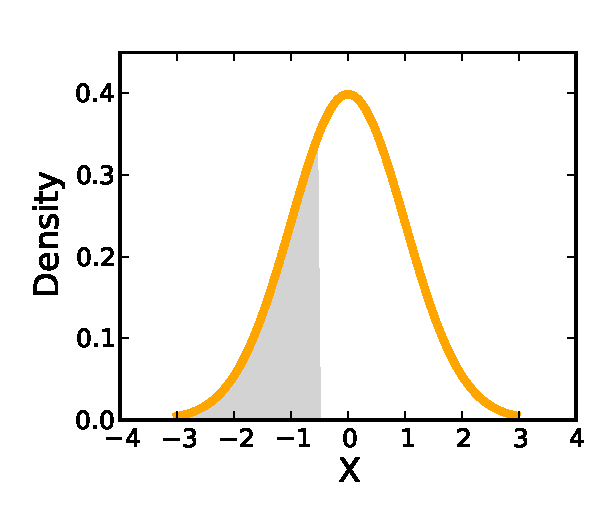
\includegraphics{000.pdf}} &
\scalebox{0.4}{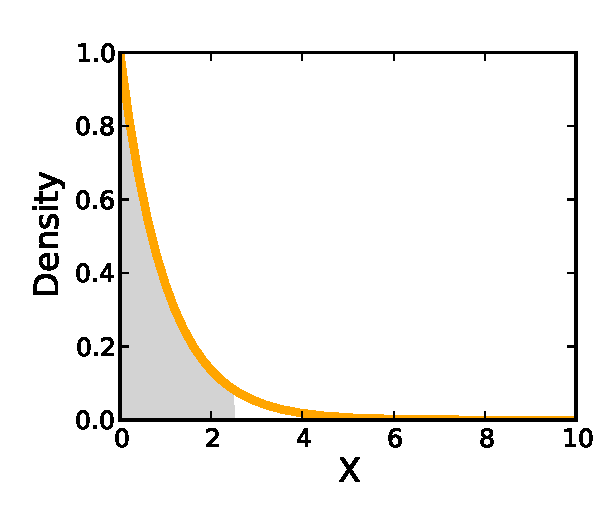
\includegraphics{001.pdf}}
\end{tabular}
\end{center}

\end{frame}

%%%%%%%%%%%%%%%%%%%%%%%%%%%%%%%%%%%%%%%%%%%%%%%%%%%%%%%%%%%
\begin{frame}
\frametitle{Characteristics of density functions}

A basic property of a density function is its {\bf location} -- the
central or most typical value.  

There are many measures of location, but by any reasonable measure the
density on the right, below, would have a greater location than the
density on the left.

\begin{center}
\begin{tabular}{cc}
\scalebox{0.4}{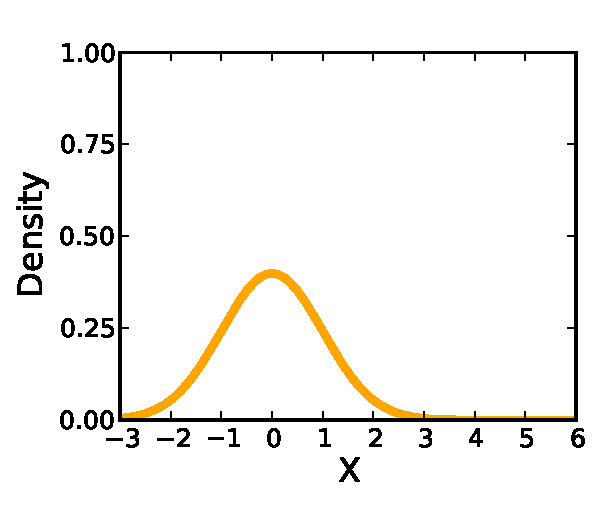
\includegraphics{002-0.pdf}}&
\scalebox{0.4}{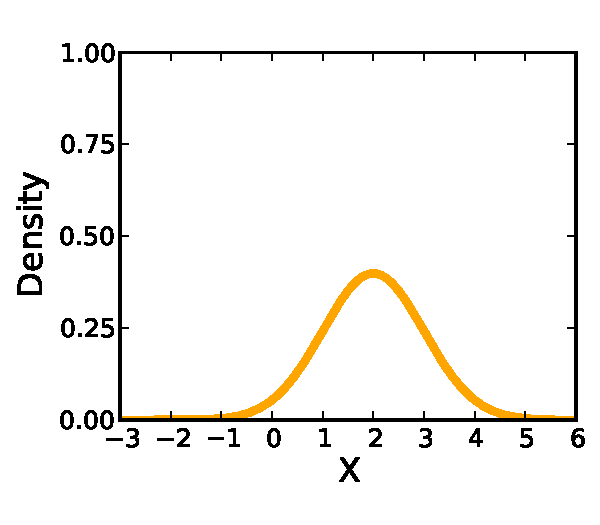
\includegraphics{002-1.pdf}}
\end{tabular}
\end{center}

\end{frame}

%%%%%%%%%%%%%%%%%%%%%%%%%%%%%%%%%%%%%%%%%%%%%%%%%%%%%%%%%%%
\begin{frame}
\frametitle{Characteristics of density functions}

Another basic property of a density function is its {\bf scale},
referring to spread or width of the distribution.  

There are many measures of scale, but by any reasonable measure the
density on the right, below, would have a greater scale than the
density on the left.

\begin{center}
\begin{tabular}{cc}
\scalebox{0.4}{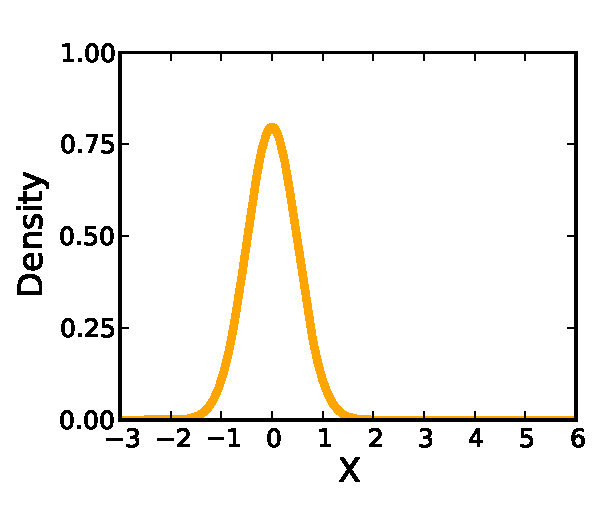
\includegraphics{002-2.pdf}}&
\scalebox{0.4}{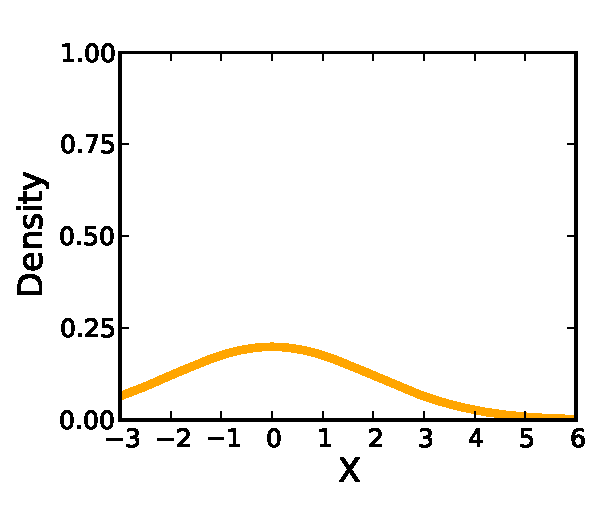
\includegraphics{002-3.pdf}}
\end{tabular}
\end{center}


\end{frame}

%%%%%%%%%%%%%%%%%%%%%%%%%%%%%%%%%%%%%%%%%%%%%%%%%%%%%%%%%%%
\begin{frame}
\frametitle{Characteristics of density functions}

Another basic property of a density function is its {\bf skew},
referring to whether one of the two tails of the density is thicker
than the other.  

The density on the left, below, is right-skewed, and the density on
the right, below, is left-skewed.


\begin{center}
\begin{tabular}{cc}
\scalebox{0.4}{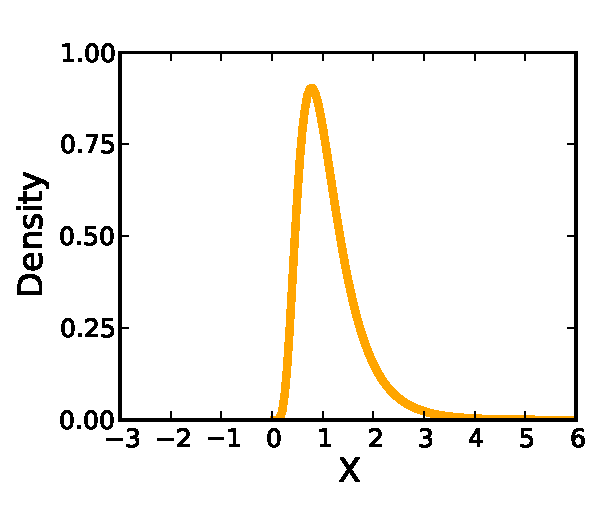
\includegraphics{002-4.pdf}}&
\scalebox{0.4}{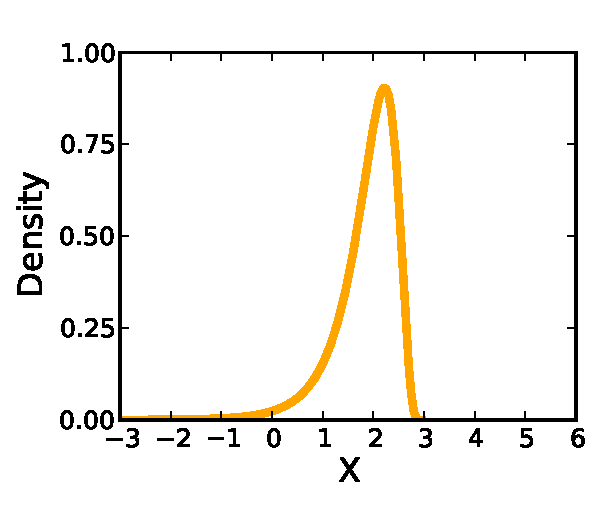
\includegraphics{002-5.pdf}}
\end{tabular}
\end{center}

%The densities on the preceding two slides are unskewed, or symmetric.

\end{frame}


